\documentclass[a4paper,11pt]{article}
\usepackage[margin=2.1cm]{geometry}
\usepackage[T1]{fontenc}
\usepackage[utf8]{inputenc}
\usepackage{lmodern,microtype,graphicx,booktabs,tabularx,array,amsmath}
\usepackage{tikz,pgfplots}
\usetikzlibrary{arrows.meta,positioning,fit}
\pgfplotsset{compat=1.18}
\usepackage{enumitem}
\usepackage{xcolor}
\definecolor{ink}{HTML}{202722}
\definecolor{accent}{HTML}{426B52}
\usepackage[colorlinks=true,allcolors=accent,breaklinks=true]{hyperref}
\usepackage{fancyhdr}
\pagestyle{fancy}\fancyhf{}
\fancyhead[L]{\small MLOps Endesa | Final report draft}
\fancyhead[R]{\small M1--M6}
\fancyfoot[C]{\thepage}
\renewcommand{\headrulewidth}{0pt}
\setlength{\headheight}{14pt}
\setlength{\parindent}{0pt}\setlength{\parskip}{0.5em}
\setlist{nosep,leftmargin=1.4em}
\setcounter{tocdepth}{2}
\newcommand{\repo}{https://github.com/mlops-2627q1-mds-upc/MLOps_Endesa}
\newcommand{\candidate}{f9b5896af998331494175733c557e8dc5dd12cc7}
\newcommand{\chartheight}{5.2cm}
\newcommand{\pr}[1]{\href{\repo/pull/#1}{PR~\##1}}
\newcommand{\file}[2]{\href{\repo/blob/\candidate/#1}{#2}}
\newcolumntype{Y}{>{\raggedright\arraybackslash}X}
\input{data-values.tex}
\hypersetup{pdftitle={MLOps Endesa: final delivery draft},pdfauthor={Team MLOps Endesa}}
\begin{document}
\begin{titlepage}
\thispagestyle{empty}
{\large UPC | Master in Data Science | Machine Learning Systems in Production\par}
\vspace{1.3cm}
{\Huge\bfseries A traceable forecasting service\par}
\vspace{0.4cm}
{\Large Electricity demand with Chronos: development, delivery and monitoring\par}
\vspace{0.8cm}
{\Large Final report | Milestones 1--6 | DRAFT\par}
12 November 2026
\vspace{0.6cm}

The implementation candidate integrates the pending release and monitoring PRs.
Human review, exact-source release execution, private publication, independent
selected-model startup and final target rollout/recovery remain open. This is a
review draft, not a submission or a completed deployment record.

\vspace{0.4cm}
\begin{tabularx}{\linewidth}{@{}lY@{}}
Repository & \href{\repo}{mlops-2627q1-mds-upc/MLOps\_Endesa} \\
Candidate & \href{\repo/tree/\candidate}{Implementation candidate f9b5896}, \pr{100}, open \\
Merged source & \href{\repo/tree/26f260e33766689bcdce4a6db6062a9e1e74475d}{main at 26f260e}; inference and API merged \\
Planning & \href{https://github.com/orgs/mlops-2627q1-mds-upc/projects/3}{Organization Project 3} \\
Data and runs & \href{https://dagshub.com/pauadal03/MLOps_Endesa}{DagsHub: DVC and MLflow} \\
Team contact & \href{mailto:pau.adal@estudiantat.upc.edu,didac.cayuela@estudiantat.upc.edu,antoni.lopera@estudiantat.upc.edu,sindri.masson@estudiantat.upc.edu,pablo.perez.cano@estudiantat.upc.edu}{Email all five members below} \\
\end{tabularx}
\vspace{0.5cm}
{\small
\begin{tabularx}{\linewidth}{@{}llYl@{}}\toprule
Surname & Name & UPC email & GitHub \\\midrule
Adal & Pau & pau.adal@estudiantat.upc.edu & pauadal03 \\
Cayuela & Dídac & didac.cayuela@estudiantat.upc.edu & didicayu \\
Lopera & Antoni & antoni.lopera@estudiantat.upc.edu & toni646 \\
Másson & Sindri & sindri.masson@estudiantat.upc.edu & sindrimasson-upc \\
Pérez Cano & Pablo & pablo.perez.cano@estudiantat.upc.edu & PabloPerezCano \\\bottomrule
\end{tabularx}}
\vfill
The supplied schedule states 14 December 2026, 23:55 for the final report and
15 December for the presentation. Atenea changes and instructor access have not
been checked for this draft.
\end{titlepage}
\tableofcontents
\clearpage
\section{Introduction}

The project compares seasonal baselines, pretrained Chronos-T5-small and a
fine-tuned checkpoint on five Australian electricity-demand series. The component
takes the 512 most recent observations for one state and forecasts 48 half-hourly
positions. The selected checkpoint is exposed through a stateless FastAPI service.
The delivery candidate adds container packaging, evidence-bound release
procedures, transactional recovery and monitoring of both service and forecasts.

The central engineering question is whether another person can identify the
exact code, data, model and settings behind a forecast, then inspect a failure
without confusing missing evidence with successful operation. The initial model
comparison has a recorded outcome. The final integrated release still needs
human review and the runtime observations described in this report.

\subsection{Goal and success criteria}

The forecasting goal was to improve equally weighted mean MASE over the untuned
model and seasonal baselines under a decision rule fixed before opening the test
block. The selected checkpoint met that historical rule: test mean MASE was
0.5571 against 0.8175 for the untuned control, 0.9885 for lag~48 and 0.9617 for
lag~336. This result concerns one selected checkpoint and one historical period;
the consumed test block is not used for further tuning.

The delivery goal is broader than a green test suite. A reviewer should be able
to retrieve the declared artifacts, start the exact model through a pinned image,
send valid and invalid requests, and observe failure and recovery with useful
monitoring. Acceptance requires a reviewed source, an exact-source validation
run, a private registry digest, independent selected-model startup and actual
target rollout/recovery evidence. These final runtime gates are pending.

Latency, calibration and drift responsiveness are measurement questions. The
historical VM and validation-subset observations below are available for human
assessment; no numerical latency or coverage SLO is adopted in this draft.
The service is for coursework and historical research, with no operational grid
scheduling claim.

\subsection{Team contribution assessment}

The initial report's equal-contribution statement applies to its own delivery.
The final-delivery consensus or CATME assessment has not been supplied. It remains
a required human team task and is not inferred from commit counts, the earlier
agreement or AI-generated text.

There is specific contribution evidence. Pablo proposed the fine-tuning options
and checked recorded runs; Sindri executed the experiments and selected option~1,
seed~8 on validation. Pau implemented the DVC/Great Expectations validation work
with Claude Code assistance. Toni reviewed the first-delivery integration;
Pablo reviewed later card updates; Dídac reviewed Pau's EDN assessment. Dídac
directed the release/monitoring implementation and this reconciliation using
Codex. These examples are supported by the experiment and merged review records;
they are not a complete allocation of final-delivery effort.

\section{Methodology}
\subsection{M1: Problem, requirements and source limits}

The data are the Australian Electricity Demand configuration of the Monash Time
Series Forecasting Archive. Five aggregate state series represent NSW, VIC, QLD,
SA and TAS. The pinned archive and DVC metadata identify the exact inputs. The
source code \texttt{QUN} is mapped to \texttt{QLD}. Each processed value remains
in the stored source scale and each row has an integer position.

The extraction package supports MW, but a specification independently confirming
the archive's physical unit has not been located. More importantly, the source
preparation places period~1 at 00:30 while TSF gives a 00:00 start string. The
project therefore uses nominal half-hourly positions. Civil-hour, DST and holiday
joins remain deferred. A general market-time convention cannot resolve the exact
archive alignment.

The common prefix contains 230,736 positions per state. Training ends at 195,696;
validation ends at 213,216; the test block ends at 230,736. QLD's additional 1,536
values and SA's additional 48 are outside that common prefix. Tasmania has 22
documented negative values, which are preserved. MAE and MASE avoid the
interpretation problems of percentage errors near zero or negative demand.

The requirements retain stable FR/NFR identifiers. The input/output contract,
artifact identity, causal contexts and training-only scaling are testable.
Requirements whose thresholds need a decision remain open. The report does not
promote measured values into policy. The dataset and model cards record
provenance, licensing, point-error results and the narrower monitoring evidence.
Data are attributed under CC BY~4.0 and Chronos under Apache~2.0.

\subsection{M1: Project coordination and communication}

The working agreement uses one accountable issue owner, short-lived task
branches, pull requests and one human peer approval. Tasks are grouped by course
milestone in the organization Project. A draft PR is not a completed task, and a
reviewable implementation can still have open runtime acceptance criteria.
The repository documents required lint/test checks, dismissed approvals after
reviewable changes and resolution of review conversations before merge.

The first-delivery integration and inference/API changes are merged. The release
and monitoring sources are integrated in the candidate with their original commit
attribution, but their individual PRs remain open. This draft has no authority to
merge them or to supply their peer review. It also leaves the already-open EDN
PR~\#97 unchanged. New decision proposals and assessments remain local text
notes for Dídac's review; pending entries are not presented as accepted decisions.

\subsection{M2: Project structure}

The repository adapts Cookiecutter Data Science: source modules, tests, notebooks,
documentation, data and model references have separate roles. Raw data and model
weights are outside Git; DVC references, dependency locks and provenance sidecars
are tracked. Generated reports, local evidence and environments are ignored.
Python~3.11 and \texttt{uv.lock} describe the main development environment.

The serving dependency group excludes notebook, DVC, MLflow and fine-tuning tools,
while preserving the imports needed by inference. Alibi Detect uses a separate
locked environment because its compatibility requirements differ from the main
project. This adds a second lock to maintain, but makes the executed detector
version explicit instead of silently changing the forecasting environment.

\subsection{M2: Code and data versioning}

Git identifies source and configuration. DVC identifies raw data, chronological
blocks and the selected model directory. The selected artifact has a versioned
weight-bound provenance sidecar that records its actual training run. A matching
directory name alone cannot establish lineage. A weights/provenance mismatch
fails loading.

The selected directory's DVC MD5 is
\texttt{0377ee21f89c25da36b95db59841c3d4.dir}. Full weights, training-run and data
identities are in the linked model card and replication guide, rather than being
copied into each result table. The validation handoff later binds those artifact
identities to source, parameters and dependency locks.

Version agreement and retrievability are different checks. Historical fresh-cache
DVC retrieval succeeded on 2 November at its recorded source. That receipt does
not establish fresh retrieval for the final candidate, Actions authentication or
an independent reviewer's permission. This document task verifies local source
setup and retrieves a small synthetic Actions evidence artifact; it does not pull
the selected weights or write shared experiment state.

\subsection{M2: Experiment tracking and model selection}

MLflow records source commit/dirty state, data and model versions, parameters,
seed, settings, metrics and artifacts. Forecast evaluation uses the same 365
origins per state: 1,825 origins and 87,600 targets per block. Origins are spaced
48 positions apart; contexts end before the origin. The lag-336 MASE denominator
is estimated from training only. State scores receive equal weight.

Chronos returns 20 sampled trajectories. The point forecast is their median;
evaluation uses sampling seed~7. Training seed and forecast-sampling seed are
separate. Fine-tuning used training windows with 512 context positions and 64
labels, all ending before the training boundary; evaluation retained its 48-step
horizon. Option~1 used 1,000 steps, AdamW and learning rate 0.001 decaying to zero.
It was selected on validation, with seed~8 selected as its checkpoint.

\begin{table}[ht]\centering
\caption{Recorded Experiment~004 comparison. Lower mean MASE is better. These
are historical measurements, not runs performed for this draft.}
\begin{tabular}{lrr}\toprule
Method & Validation & Test \\\midrule
Selected fine-tuned, option~1 / seed~8 & 0.5649 & 0.5571 \\
Untuned Chronos control, GPU & 0.8737 & 0.8175 \\
Seasonal naive, lag~48 & 1.0422 & 0.9885 \\
Seasonal naive, lag~336 & 1.2020 & 0.9617 \\\bottomrule
\end{tabular}\end{table}

The decision margin, 0.0091, was fixed before opening test. It is option~1's
validation seed range, not a confidence interval or significance threshold. The
selected model's test MASE is 31.9\% below the GPU control and 43.6\% below lag~48.
Its error is more concentrated in the worst origins: worst-5\% error share 0.183,
against 0.147 for the control. The lower mean does not remove that limitation.

\subsection{M3: Energy efficiency awareness}

CodeCarbon and GPU NVML power samples estimate energy; these are not wattmeter
measurements. The selected training run took about 678 seconds and 0.0276~kWh
on an RTX~4060 with 8~GB. Across 37 measured training/evaluation runs, the total
was 1.126~kWh and about 196~g CO\textsubscript{2}eq. One timed-out evaluation had
no energy record and is excluded from that total.

About 0.51~kWh of the measured cost was avoidable GPU-memory-related evaluation
overhead. Failed and slow attempts remain in Experiment~004 rather than being
removed from the accounting. Serving energy is still unmeasured. Lower compute
time on a different machine cannot be substituted for a serving-energy result.

\subsection{M3: Static analysis and data/model testing}

Required CI runs Ruff formatting/lint, notebook checks, Pylint and pytest with
statement/branch coverage. No coverage percentage threshold has been adopted.
The candidate's exact-head CI reported 1,037 passes, 109 skips and 82\% rounded
coverage. The checks ran against GitHub's generated PR merge; their source head
and actual checkout identity are retained separately. The skips include optional
data/model/backend cases and are not passing model executions.

Data validation combines 74 Great Expectations expectations with 44 Python checks,
118 aggregate checks in total. It checks schema, complete indexes, origin grids,
finite values and the documented TAS negatives. Training-derived ranges avoid
fitting bounds to validation or test. The held-out structure can be inspected
without scoring or tuning the model on its targets.

Behaviour cases fix their expected patterns and limits before inference. The
selected checkpoint's separate October record contains 10/10 minimum-functionality
cases, 70/70 invariance pairs and 12/12 directional cases plus an unchanged control
passing the declared limits. An interrupted four-thread attempt was retained,
then a two-thread configuration was used. These bounded synthetic and
training/validation tests do not establish arbitrary-input robustness.

\subsection{M4: System design and serving environment}

The architecture separates online inference, release control and offline replay
(Figure~\ref{fig:architecture}). FastAPI loads one verified predictor at startup.
There is no training endpoint, automatic model reload or base-model fallback.
The API has no persistent request history; the replay client records its own
forecast requests and progressively released observations in SQLite.

\begin{figure}[ht]\centering
\resizebox{\linewidth}{!}{%
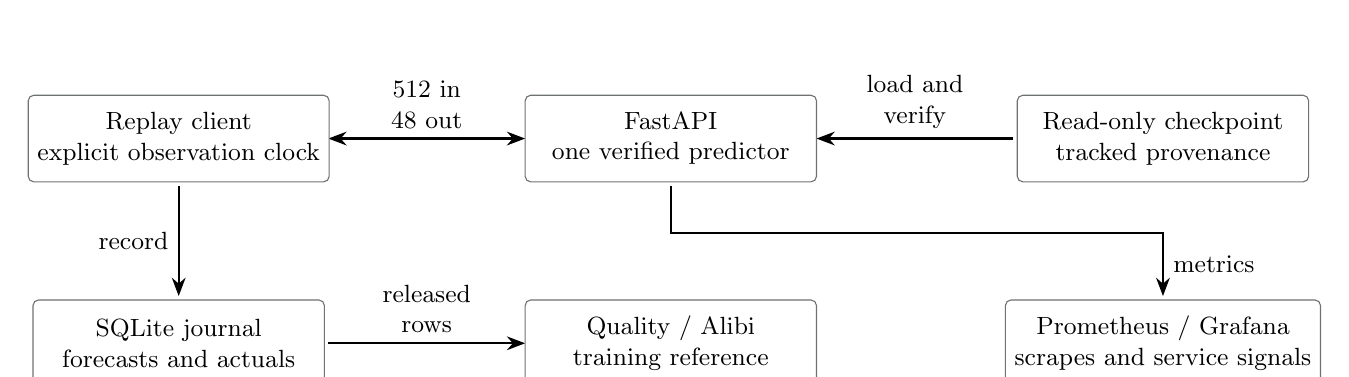
\begin{tikzpicture}[font=\small,>=Stealth,
  box/.style={draw=ink!65,rounded corners=2pt,align=center,minimum width=3.7cm,minimum height=1.1cm,fill=white}]
\draw[<->,thick] (1.9,0) -- node[above,align=center]{512 in\\48 out} (4.4,0);
\draw[->,thick] (10.6,0) -- node[above,align=center]{load and\\verify} (8.1,0);
\draw[->,thick] (0,-.6) -- node[left]{record} (0,-2.0);
\draw[->,thick] (1.9,-2.6) -- node[above,align=center]{released\\rows} (4.4,-2.6);
\draw[->,thick] (6.25,-.6) -- (6.25,-1.2) -- (12.5,-1.2) -- node[right]{metrics} (12.5,-2.0);
\node[box] at (0,0) {Replay client\\explicit observation clock};
\node[box] at (6.25,0) {FastAPI\\one verified predictor};
\node[box] at (12.5,0) {Read-only checkpoint\\tracked provenance};
\node[box] at (0,-2.6) {SQLite journal\\forecasts and actuals};
\node[box] at (6.25,-2.6) {Quality / Alibi\\training reference};
\node[box] at (12.5,-2.6) {Prometheus / Grafana\\scrapes and service signals};
\end{tikzpicture}}

\caption{Implemented interfaces in the candidate. Solid arrows are forecast,
scrape or journal data flows. The release controller prepares/verifies the API
slot separately. The diagram describes source structure, not a verified final
target deployment.}\label{fig:architecture}
\end{figure}

The intended target is the allocated FIB Virtech Linux amd64 VM. Local Mac checks,
an amd64 image under emulation and native Linux CI each answer different
questions. Target preparation binds VM allocation, host key, guest hostname,
machine ID, account and local Docker socket before touching a service. Image,
model and parameter identities belong to separate read-only slots. Installed
resources, model/data caches, previous containers and trusted evidence are
preserved.

The deployment helper uses one worker and two numerical threads. Readiness has a
90-second bound; requests have 30-second bounds. These are procedure budgets,
not forecast latency SLOs. The final source/image/model combination has not been
observed on the target. UPC/VPN-dependent work is halted until the user supplies
the required access step; this draft task initiates no VPN, SSH or tunnel.

\subsection{M4: API contract and failure behaviour}

\texttt{POST /forecast} accepts only a known state and exactly 512 finite JSON
numbers, oldest first. Booleans, strings, nulls, unknown states and non-finite or
out-of-float32-range values are rejected. Valid negatives are preserved. The state
labels requests and monitoring; it is not a model feature or a separate-model
selector.

A success returns 48 finite values for each of p10, p50 and p90, ordered at every
position, plus the actual weights revision, training run, source scale and executed
sampling settings. Nominal p10/p90 quantiles do not promise empirical 80\% coverage.
The service makes no inferred timestamp or unit conversion.

\begin{table}[ht]\centering
\caption{Public HTTP distinctions used by tests and later release checks.}
\begin{tabularx}{\linewidth}{lY}\toprule
Observation & Meaning \\\midrule
\texttt{/health}: 200 & Process responds; no model inference. \\
\texttt{/ready}: 200 & Predictor loaded; does not prove every input succeeds. \\
\texttt{/forecast}: 200 & A forecast passed shape/value/identity validation. \\
Invalid request: 422 & Strict public input contract rejected the request. \\
Unavailable/prediction error: 503 & Model unavailable or forecast failed; no fallback. \\
Invalid model output: 500 & Predictor violated output shape, ordering or identity. \\\bottomrule
\end{tabularx}\end{table}

Endpoint tests use an injected factory through the production lifespan. The test
factory is a Python argument and cannot be selected through deployment settings.
A historical selected-model HTTP smoke on 23 October returned matching ordered
forecasts twice and refused startup with missing weights. Those local checks
retain their own source and hardware; they do not qualify a final container.

\subsection{M5: Container packaging}

The Dockerfile pins Python/uv base versions and multi-architecture digests. The
release workflow targets Linux amd64; base-image architecture support does not
qualify every complete serving platform. Packages are installed from the locked
CPU serving group. The production image contains explicit runtime sources,
parameters and provenance, but no weights, data, credentials, development
environment or fixture predictor. The context allowlist makes this exclusion
testable.

The process runs as UID/GID~10001, one worker, with a read-only root, a bounded
temporary filesystem and a read-only selected-model mount. Startup hashes the
weights against provenance; absent or mismatched weights abort. The image's
source label identifies the declared build commit, which still requires a clean
matching build context.

Native-amd64 container CI checks CPU imports, non-root execution and the normal
missing-weight failure, then starts a separately mounted synthetic factory for
HTTP 200/200/200/422 checks. Its \texttt{fixture\_only} result is explicit. The
fresh local scenarios use an inspected cached fixture image with a read-only
source overlay under Mac emulation. Neither produces a final-source image or
loads the selected checkpoint.

\subsection{M5: CI/CD and release recovery}

Ordinary PR checks are automatic; real-model release validation and publication
are manual workflows with reviewed prerequisites. The bounded validator retrieves
the declared DVC artifacts, checks complete identities, configures private GX
resources, validates data and executes existing minimum-functionality/directional
cases sequentially. Total runtime is capped at 900 seconds. It neither trains nor
repeats the consumed final-test comparison.

Its public handoff binds source/tree/dirty state, data, complete model directory,
weights/training run, configuration, dependency lock, run/attempt and detailed
report hashes. Publication selects the authenticated successful Actions
run/attempt/artifact for the exact source and verifies archive bytes and complete
reports before building. A similar tree or a successful run for another commit
cannot authorize publication.

The selected registry is private GHCR. Source restricts the destination and
checks package identity/visibility. First-publication bootstrap is explicit and
off by default. A 404 records unobserved existence/access, not proven absence.
Post-push private metadata is required before a release can succeed. This guard
does not change settings, establish reader rights or lock future visibility.
No package publication occurred for this candidate.

The target transaction takes a persistent exclusive lock and verifies the accepted
baseline before a candidate stop/start. It durably records pending identities,
requires the baseline to stop cleanly, then checks the candidate. On success it
advances current and retains previous. On candidate failure it attempts recovery
of the accepted baseline and records restored forecast evidence. Failure remains
exit~1 even when recovery succeeds. An expected-current fence rejects stale
operators. Recorded current/previous/pending/generation is state, not target health.

Workflow semantics are checked separately with actionlint. A real earlier Actions
failure used an unavailable \texttt{runner} context in job-level environment
configuration, despite passing YAML/bash checks. Moving the value into a runner
step fixed that source error; the invalid-context regression remains. Semantic
checks still do not prove a publication workflow has executed.

\subsection{M6: Resource and service monitoring}

The API exposes request counts, status classes, completed-request durations,
in-flight forecasts, readiness and process CPU/RSS availability. Labels are
bounded. Absence is not represented as zero work. Linux process collection and
container cgroup memory are distinct scopes; Mac process-collector gaps do not
establish missing Linux telemetry. Prometheus/Grafana configuration and promtool
tests cover scrape, readiness and missing-series states.

The historical 2 November VM benchmark ran discovery and confirmation with
47 forecasts each and no HTTP errors. Warm c1 p95 was 4.791 and 5.028 seconds;
c2 p95 was 9.189 and 9.363 seconds, while throughput stayed around 0.22 requests/s.
Figure~\ref{fig:latency} uses the retained measurement manifest. Each warm phase
has 20 requests. The result suggests queueing under that configuration; it does
not establish maximum capacity, admission control or an adopted latency target.

\begin{figure}[ht]\centering
\begin{tikzpicture}
\begin{axis}[width=.94\linewidth,height=\chartheight,ymin=0,ymax=11,
  ybar,bar width=24pt,xtick={0,1},xticklabels={Concurrency 1,Concurrency 2},
  ylabel={Warm p95 (seconds)},ytick={0,2,4,6,8,10},
  xmin=-.6,xmax=1.6,axis x line*=bottom,axis y line*=left,
  ymajorgrids=true,grid style={gray!20},
  tick label style={font=\small},label style={font=\small},
  legend columns=2,
  legend style={font=\small,draw=none,at={(.5,1.02)},anchor=south},
  nodes near coords,nodes near coords style={font=\small,/pgf/number format/fixed,/pgf/number format/precision=2}]
\addplot[fill=ink!80,draw=ink!80] table[x=index,y=discovery,col sep=comma]{latency.csv};
\addplot[fill=accent!65,draw=accent] table[x=index,y=confirmation,col sep=comma]{latency.csv};
\legend{Discovery,Confirmation}
\end{axis}
\end{tikzpicture}

\caption{Historical selected-model VM experiment: warm p95 response time, seconds,
from 20 requests per phase. One guest CPU, a 2~GiB container cap and one retained
synthetic TAS history. Source/image differ from the final release; discovery and
confirmation are small experiments, not uncertainty intervals.}\label{fig:latency}
\end{figure}

The recorded container high-water maximum was about 1.266~GiB; host memory was
not measured. Both one-second stops ended with exit~137, \texttt{OOMKilled=false}
and zero recorded OOM/failure counters. This establishes neither graceful stop
nor OOM. The protected main API remained available in those historical receipts.

Fresh 12 November isolated HTTP/Prometheus evidence is narrower but direct. The
normal control had no active alerts. Stopping only the owned synthetic API caused
\texttt{ForecastApiDown} to fire \OutageDelay{} seconds after fault onset, with
the original one-minute hold unchanged. It cleared after restart and a subsequent
forecast returned 200 (Figure~\ref{fig:outage}). The isolated scrape/evaluation
intervals were two seconds. No external notification receiver is configured.

\begin{figure}[ht]\centering
\resizebox{.98\linewidth}{!}{%
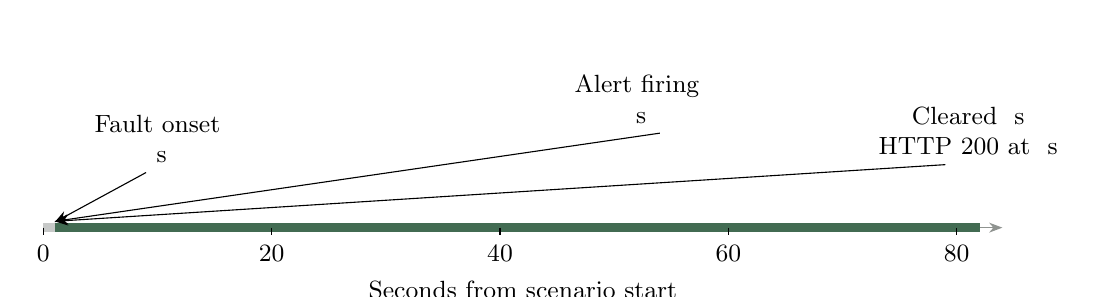
\begin{tikzpicture}[x=.145cm,y=1cm,font=\small,>=Stealth]
\draw[->,ink!50] (0,0) -- (84,0);
\draw[line width=3pt,ink!25] (0,0) -- (\OutageStart,0);
\draw[line width=3pt,orange!65!black] (\OutageStart,0) -- (\OutageFire,0);
\draw[line width=3pt,red!65!black] (\OutageFire,0) -- (\OutageClear,0);
\draw[line width=3pt,accent] (\OutageClear,0) -- (82,0);
\foreach \x in {0,20,40,60,80}{\draw (\x,0) -- (\x,-.09);\node[below] at (\x,-.1){\x};}
\node[below] at (42,-.55){Seconds from scenario start};
\draw[->] (9,.7) -- (\OutageStart,.07);
\node[above,align=center] at (10,.7){Fault onset\\\OutageStart{} s};
\draw[->] (54,1.2) -- (\OutageFire,.08);
\node[above,align=center] at (52,1.2){Alert firing\\\OutageFire{} s};
\draw[->] (79,.8) -- (\OutageClear,.08);
\node[above,align=center] at (81,.8){Cleared \OutageClear{} s\\HTTP 200 at \OutageHttp{} s};
\end{tikzpicture}}

\caption{Actual isolated local outage: seconds from scenario start. Marks identify
fault onset, firing, clearing and recovered HTTP. A synthetic predictor ran in
an owned cached amd64 fixture image under Mac emulation. This is not target
deployment or notification-delivery evidence.}\label{fig:outage}
\end{figure}

Three slow synthetic requests returned 200 in 0.257--0.265 seconds, followed by
0.004-second recovery. That checks duration collection around a declared
0.25-second delay. It is not a real-model benchmark or a configured latency alert.
Two failed procedures remain retained: one recovery used a stale Docker port;
the fix refreshes bindings and the client. Another slow attempt returned 503;
atomic fault publication/read-back preceded a passing rerun, but the original
predictor exception is unknown. Failed runs were not relabelled as successes.

\subsection{M6: Model performance and chronological monitoring}

The replay client records forecasts, model/settings/source identities and
progressively released actuals in SQLite. It reads only training/validation
artifacts matching the recorded identities. A target at position $t$ is usable
only after its declared observation-release clock. Forecast steps and unique
state/target pairs are different denominators when origins overlap.

The quality consumer reuses training-only lag-336 MASE scales and the stored
lag-48 comparison. It reports MAE, MASE, empirical p10/p90 coverage, mean interval
width, pending joins and per-state/horizon sample status. The default minimum is
30 matched rows per group, set before execution. Missing truth or insufficient
samples produce explicit states rather than zero error or an apparently healthy
dashboard. Report freshness is separate from forecast quality.

In the fresh delayed-observation fixture, clock~516 had 6 matched and 186 pending
forecast steps. Releasing through clock~563 produced 192 matches and zero pending.
The fixture's display minimum of two illustrates the transition; default
minimum-30 horizon groups remained insufficient. These synthetic perfect
intervals cannot estimate selected-model calibration.

The historical selected-model validation subset has 30 origins per state,
150 forecasts and 7,200 released joins. Figure~\ref{fig:coverage} shows empirical
coverage from 61.25\% to 74.93\%, below nominal 80\% for every state. There are
30 rows per state/horizon and dependence within forecasting sequences. This is a
bounded subset, not complete validation calibration, and no coverage threshold or
automatic corrective action has been adopted.

\begin{figure}[ht]\centering
\begin{tikzpicture}
\begin{axis}[width=.94\linewidth,height=\chartheight,ymin=0,ymax=100,
  ybar,bar width=22pt,xtick={0,1,2,3,4},xticklabels={NSW,VIC,QLD,SA,TAS},
  ylabel={Empirical coverage (\%)},ytick={0,20,40,60,80,100},
  xmin=-.6,xmax=4.6,axis x line*=bottom,axis y line*=left,
  ymajorgrids=true,grid style={gray!20},tick label style={font=\small},
  label style={font=\small},enlarge x limits=false]
\addplot[fill=accent,draw=accent,point meta=y,nodes near coords,
 nodes near coords style={font=\small,/pgf/number format/fixed,/pgf/number format/precision=1}]
 table[x=index,y=coverage,col sep=comma]{coverage.csv};
\addplot[sharp plot,dashed,thick,ink,forget plot] coordinates {(-.6,80) (4.6,80)};
\node[anchor=south east,font=\small] at (axis cs:4.55,82) {Nominal 80\%};
\end{axis}
\end{tikzpicture}

\caption{Historical selected-model p10/p90 coverage on 30 validation origins per
state (1,440 steps/state). The dashed line is nominal 80\%, not an adopted SLO.
Percentages are drawn directly from the versioned subset summary.}\label{fig:coverage}
\end{figure}

Alibi Detect compares weekly-residual features against 104 complete training
cycles. Each tested window needs eight full weekly cycles: 2,688 half-hourly
positions, or 56 nominal days. Reference, configuration, multiple-testing budget
and sample completeness are fixed. The historical validation control raised
8/30 state-window alarms; natural changes may exist, so this is a false-alert
proxy. First detection of declared level/variability shifts took 56--112 nominal
days, with missed windows retained. Those results do not support a rapid live
detection claim.

The fresh synthetic Alibi run is separate from historical playback. All five
states produced no-drift control at position~37,632, drift after a fixed level
shift at 40,320 and no-drift restored distribution at 43,008, with no missed shift
windows or control/recovery alarms in that declared run. The roughly three-second
compressed execution time is not live detection latency. Recovery is the next
scheduled statistical result, not an operational alert reset. Neither a drift
result nor a low-coverage subset triggers automatic retraining.

\section{Self-evaluation of the project}

The model experiment has a clear result and traceable limitations. The selected
checkpoint lowered mean error under a predeclared test rule, but interval
calibration and concentration of worst-origin errors remain weaker areas. The
archive's unresolved clock prevented a defensible holiday analysis. Preserving
that limit was preferable to silently assigning a convenient timestamp mapping.

The release work exposed a different issue: evidence must follow the exact source
and environment. A local model smoke, a native container fixture, a historical VM
benchmark and a passing workflow-semantic check do not together establish a
published final release. The candidate makes those identities explicit, but the
operational chain still needs actual execution and human review.

The retained failures provide concrete lessons. A one-second container stop is
not a graceful-stop demonstration. A restarted container can change its dynamic
port, so recovery must inspect its actual binding. File-based fault control needs
atomic publication and acknowledgment. YAML syntax alone does not validate
GitHub expression contexts. The associated corrections were implemented and
checked; their original failures remain available for review.

If repeating the project, earlier definition of the artifact handoff, final
runtime access and small-sample monitoring limitations would reduce late
integration work. Drift needs a usefulness assessment: 56-day windows can
support a course experiment while being unsuitable for a rapid response goal.
Additional observations should follow declared policies, rather than tuning the
frozen test comparison or selecting thresholds after seeing failures.

The implementation uses chronological evaluation, distribution testing and
transactional persistence. Connections to specifically named prior courses are
awaiting team input; no course attendance or personal learning experience is
invented here. The final consensus/CATME assessment, approved EDN annex, human
rehearsal, reviewer access and Atenea confirmation also remain open.

\subsection{Actual AI assistance}

AI assistance was substantive. Earlier records attribute source investigation,
alternative comparison, evaluator and test-runner implementation, provenance
repair and documentation to Codex, and initial report and data-validation
implementation assistance to Claude Code. Sindri ran the fine-tuning experiments
and chose seed~8 on validation after AI initially suggested seed~7. The human
choice and recorded peer reviews remain separate from the AI work.

For the release/monitoring candidate, Codex implemented helpers, fixtures,
workflow safeguards, monitoring consumers and scenario procedures under Dídac's
direction, and helped examine retained local/runtime evidence. This draft used
Codex to reconcile source/PR identities, write and revise prose, create editable
diagrams/charts, prepare the build and inspect rendered outputs. Human final
review, contribution assessment and acceptance of proposed decisions remain
pending. The disclosure covers implementation, testing, evidence analysis and writing.
Course-prescribed use of MLflow, DVC or Alibi is not itself an AI-use disclosure.

\subsection{Delivery status and next execution}

The implementation source is pinned and the report/presentation are rebuildable
drafts. Required peer reviews and merges come first. A later authorized execution
must validate the exact reviewed release in Actions, publish/check the private
digest, prove independent selected-model startup, then perform target
rollout/recovery with a verified published baseline and fresh monitoring. Work
requiring UPC/VPN waits for the user. The final checklist is linked in Annex~B;
none of those remaining steps is inferred from this report build.

For this draft, an artifact-free source export installed the development
environment successfully using the locked dependencies already cached on the Mac.
Its focused API/scenario suite passed 113 tests; the actual-Alibi case was
intentionally excluded from that main environment. The separate earlier Actions
job supplies its own real synthetic-KS evidence. Repository lint passed with
Pylint~9.74; documentation links and figure inputs were checked separately.

A small synthetic Alibi evidence artifact was retrieved from the exact candidate's
successful Actions run through Dídac's authenticated GitHub access. Its archive
digest matched the API metadata. This verifies access to that unexpired evidence
artifact only. No selected-model/data DVC pull, private image retrieval,
independent reviewer access or target connection was attempted. Both document
PDFs passed structural checks and were rendered for page/slide inspection; the
15-minute timings remain a plan awaiting a human rehearsal.

\label{endmain}
\clearpage\appendix
\section{Engineering Decision Notebook status and sources}

The formal merged notebook contains EDN-001 through EDN-012. It records workflow,
tracking, bounded comparison, source limits, energy, CI, archive integrity, data
validation, behavioural testing and fine-tuning choices. The
\file{docs/edn/README.md}{formal EDN index} links their full decision, participant,
AI-involvement, response and assessment fields.

\pr{97} is an existing pending proposal at its own source and remains unchanged.
Further decision drafts stay in ignored local text files for Dídac's review. This
annex does not copy pending entry text, assign final numbers, fabricate human
assessments or claim acceptance. Before submission, the user must approve the
applicable decisions and final annex in the form required by the course.

The draft follows the supplied MLOps laboratory slides: report structure on
slides~13--15, M4--M6 criteria on slides~28, 30 and~32, presentation/delivery
instructions on slides~33--34 and practice weights/EDN/individual assessment on
slides~36--41. The 30-page report limit excludes annexes. Available local
repository/report review notes were read; no separate final instructor assessment
was found or invented. The source corpus included the initial report's editable
TeX and the supplied initial PDF presentation; originals were preserved.

\begin{tabularx}{\linewidth}{@{}lY@{}}\toprule
Record & Direct source at the implementation candidate \\\midrule
Problem, units and model & \file{docs/requirements.md}{Requirements},
\file{docs/DATASET_CARD.md}{dataset card}, \file{docs/MODEL_CARD.md}{model card} \\
Training and testing & \file{docs/experiments/004-chronos-fine-tuning.md}{Experiment 004},
\file{docs/experiments/008-selected-checkpoint-behaviour.md}{Experiment 008} \\
Serving and release & \file{docs/api.md}{API}, \file{docs/container.md}{container},
\file{docs/release-validation.md}{release validation},
\file{docs/image-publication.md}{publication},
\file{docs/deployment-release.md}{transactions} \\
Monitoring and observations & \file{docs/experiments/009-serving-benchmark.md}{VM benchmark},
\file{docs/replay.md}{replay}, \file{docs/drift.md}{drift},
\file{docs/forecast-quality.md}{quality},
\file{docs/monitoring-scenarios.md}{local scenarios} \\
Primary references & \href{https://arxiv.org/abs/2403.07815}{Ansari et al. (2024), Chronos};
\href{https://arxiv.org/abs/2105.06643}{Godahewa et al. (2021), Monash archive};
\href{https://zenodo.org/records/4659727}{Australian electricity archive} \\\bottomrule
\end{tabularx}

\clearpage
\section{Replication and reviewer checklist}

The tracked \href{\repo/tree/docs/85-final-delivery/docs/delivery}{delivery sources}
contain a local build script and a 900-second speaker guide. The script reads
versioned figure data, builds both PDFs sequentially and writes an output/source
manifest. The report and deck identify the implementation candidate separately
from their documentation source. Generated PDFs/ZIPs and unreviewed decision
notes stay ignored and local.

\begin{enumerate}
\item Read the immutable candidate and focused documentation diff. Confirm human
peer review and actual merged state; the source ledger lists every dependency.
\item Follow \file{docs/replication.md}{replication} for locked setup, fast checks,
data/model identities and the separate optional model route. A populated cache
does not prove remote artifact access.
\item Confirm reviewer GitHub/Project, DagsHub DVC/MLflow and future private GHCR
rights from the reviewers' own accounts; share no credentials. Access from one
author's account cannot establish instructor access.
\item Obtain a clean exact-source Actions validation with fresh authenticated
retrieval, then a trusted successful publication manifest/digest and independent
native-amd64 selected-model startup. Historical runs and small synthetic evidence
downloads do not satisfy these gates.
\item After the user supplies any required UPC/VPN step and authorizes the concrete
execution, prove target identity/capacity, adopt a verified published baseline,
execute one fenced transaction and observe restored forecasts plus fresh scrapes.
Keep one worker/two threads and bounded readiness/requests/scenarios.
\item Complete human decisions, final contribution/CATME, approved EDN annex and
prior-course connections. Rebuild/inspect the revised PDFs, rehearse 15 minutes,
confirm Atenea dates and instructor access. Submit/tag/publish only after explicit
authorization.
\end{enumerate}
\end{document}
